% vim: set spell:
\documentclass{sigchi-ext}
% Please be sure that you have the dependencies (i.e., additional
% LaTeX packages) to compile this example.
\usepackage[T1]{fontenc}
\usepackage{textcomp}
\usepackage[scaled=.92]{helvet} % for proper fonts
\usepackage{graphicx} % for EPS use the graphics package instead
\usepackage{balance}  % for useful for balancing the last columns
\usepackage{booktabs} % for pretty table rules
\usepackage{ccicons}  % for Creative Commons citation icons
\usepackage{ragged2e} % for tighter hyphenation

% \usepackage{marginnote} \usepackage[shortlabels]{enumitem}
% \usepackage{paralist}

% EXAMPLE BEGIN -- HOW TO OVERRIDE THE DEFAULT COPYRIGHT STRIP --
 \copyrightinfo{Permission to make digital or hard copies of all or
 part of this work for personal or classroom use is granted without
 fee provided that copies are not made or distributed for profit or
 commercial advantage and that copies bear this notice and the full
 citation on the first page. Copyrights for components of this work
 owned by others than ACM must be honored. Abstracting with credit is
 permitted. To copy otherwise, or republish, to post on servers or to
 redistribute to lists, requires prior specific permission and/or a
 fee. Request permissions from permissions@acm.org.\\
 {\emph{CHI'14}}, April 26--May 1, 2014, Toronto, Canada. \\
 Copyright \copyright~2014 ACM ISBN/14/04...\$15.00. \\
 DOI string from ACM form confirmation}
% EXAMPLE END

\title{Study Social: Mobile Application For Study Group Formation and Collaboration}



\numberofauthors{4}
% Notice how author names are alternately typesetted to appear ordered
% in 2-column format; i.e., the first 4 autors on the first column and
% the other 4 auhors on the second column. Actually, it's up to you to
% strictly adhere to this author notation.
\author{%
  \alignauthor{%
    \textbf{Kai Anderson}\\
    \affaddr{Utah State University} \\
    \affaddr{Logan, UT 84321, USA} \\
    \affaddr{kai.andersom@gmail.com} }\alignauthor{%
    \textbf{Erik Falor}\\
    \affaddr{Utah State University} \\
    \affaddr{Logan, UT 84321, USA} \\
    \email{ewfalor@gmail.com} } \vfil \alignauthor{%
    \textbf{Maur\'{i}el Ramirez}\\
    \affaddr{Utah State University} \\
    \affaddr{Logan, UT 84321, USA} \\
    \email{mauriel.ramirez@gmail.com} }\alignauthor{%
    \textbf{Alan Williams}\\
    \affaddr{Utah State University} \\
    \affaddr{Logan, UT 84321, USA} \\
    \email{alan.williams@aggiemail.usu.edu} } \vfil  }




% Paper metadata (use plain text, for PDF inclusion and later
% re-using, if desired)
\def\plaintitle{Study Social: Forming Study Groups Online Through Social Media} \def\plainauthor{Kai Anderson, Erik Falor, Maur\'{i}el Ramirez, Alan Williams}
\def\plainkeywords{
	Social Media; Study Groups; Study Habits; Dating Service}
\def\plaingeneralterms{Documentation, Standardization}

%% Set up our PDF with metadata
\hypersetup{%
  pdftitle={\plaintitle}, pdfauthor={\plainauthor},
  pdfkeywords={\plainkeywords}, }

% \reversemarginpar%

\begin{document}

\maketitle

% Uncomment to disable hyphenation (not recommended)
% https://twitter.com/anjirokhan/status/546046683331973120
\RaggedRight{}

% Do not change the page size or page settings.
\begin{abstract}

Study Social is a mobile application which brings students together for
collaborative work and study. There are many well-established benefits to
group study, including reduced procrastination, improved recall, exposure
to other perspectives, and more success at overcoming challenging material.
Despite these benefits students are hesitant to form new groups for myriad
reasons.  Study Social is a complete solution for students seeking group
collaboration experiences by overcoming social barriers.  In this paper we
describe our design goals and testing methodology of the Study Social
application.

\end{abstract}

\keywords{\plainkeywords}

\category{H.1.2}{User/Machine Systems}{Human factors, Software psychology}
\category{H.5.2}{User Interfaces}{Graphical user interfaces, prototyping, User-centered design, Interaction styles}
\category{H.5.3}{Groups and Organization Interfaces}{Asynchronous interaction, Collaborative computing, Computer-supported cooperative work, Organizational design, Web-based interaction}

\section{Introduction}

The genesis of the Study Social application was the identification by our group of the
need among university students of a tool for in support of collaboration and group study. 

While this software has a broad application, the initial purpose was to
help students form and find study groups composed of compatible classmates.
Beyond finding groups, the Study Social application assists group members 
with organizational tasks through communication tools such as chat rooms and
message boards, along with an integrated search interface, user profiles, 
endorsements and file uploads.

\subsection{Problem Statement}

Our initial problem statement when we began our research was, ``College
students seeking a compatible study group or tutor face a challenge as
difficult as finding a date''. While the initial problem statement is still
valid, helping students form groups and collaborate with as-yet acquainted
classmates proves to be much more complicated.

Our initial research into student study habits and previous study 
group experiences revealed that many university students are hesitant to join
a study group on their own accord due to negative experiences in group settings.
The result is that participants reported a strong preference to work through
difficult material by themselves rather than join a study group. Reported barriers
include: large groups tend to socialize instead of study, group
members with had different levels of motivation fail to expend equal effort,
mismatched knowledge levels between participants lead to confusion or frustration,
and widespread dissatisfaction with study groups mandated by the instructor.
In general our study participants reported instances of good group study outcomes,
but the recollection of negative experiences loomed large in their minds.

Research by Petress indicates the benefits of group study as: increases confidence,
improves student's subject articulation, broadens perspective, validates
knowledge, etc. \cite{petress2004benefits}. In order to make a successful
application we began our work overcoming social barriers to forming a group
while creating a tool to help students take advantage of the benefits of group
study. Creating a platform to include setting up a profile for interactions,
finding a group (joining or creating a group), interacting with the group in a
meaningful ways (events, chat, and file upload).



\section{Literature Review}
Through the development of Study Social our design gained insights from
previous research on context-aware matching, relevant feed algorithms,
understanding motivation for dating sites, tutor overuse burnout, etc as well
as our own market research.

Krzywicki's ``Interaction-based collaborative filtering methods for
recommendation in online dating''~\cite{krzywicki2010interaction} which is
relevant in matching students in tutor situations. The idea behind
Krzywicki's research is there will be a burnout for popular users and the
less popular will not receive interactions.  To avoid this type of negative
matching system we are focusing on group's as a middle ground and users will
not seek other users directly.

Lommatzsch's ``Real-time recommendations for user-item
streams''~\cite{lommatzsch2015real} provides insights into serving relevant
information feeds. While not yet implemented in Study Social this information
is key to the ``Around Me'' group feed featured in the prototype.

``Too much information'' by Christensen et. al.~\cite{christensen2006too}
describes a location-based content matching system. As study groups will be
comprised classmates attending the same campus, it makes sense for the
application to be aware of and to exploit geolocation technology to restrict
search results based upon physical location. 

From Petress's research on ``The Benefits of Group
Study''~\cite{petress2004benefits} we can understand the need for a platform to
facilitate group study. Market research has shown there is no major platform of
this type to directly facilitate study group formations. A few outlying
services include Google Docs to collaborate worksheets, Linked In to make
professional connections, Canvas for contacting classmates within the same
section, and other social services like Facebook for group formation.




\section{Investigative Research}


Once it was agreed to focus on just reaching out to aid university students
to connect socially within study groups, it was needed to make sure that
this idea was appropriate given a typical user's needs. This process
consisted of creating an interview rubric to help determine the
conventional feelings of students, followed by administering interviews,
then altering the purpose of the proposed tool to reach and fulfill the
needs of the individuals that would be using the application.

\begin{marginfigure}[-10pc]
  \begin{minipage}{\marginparwidth}
    \centering
    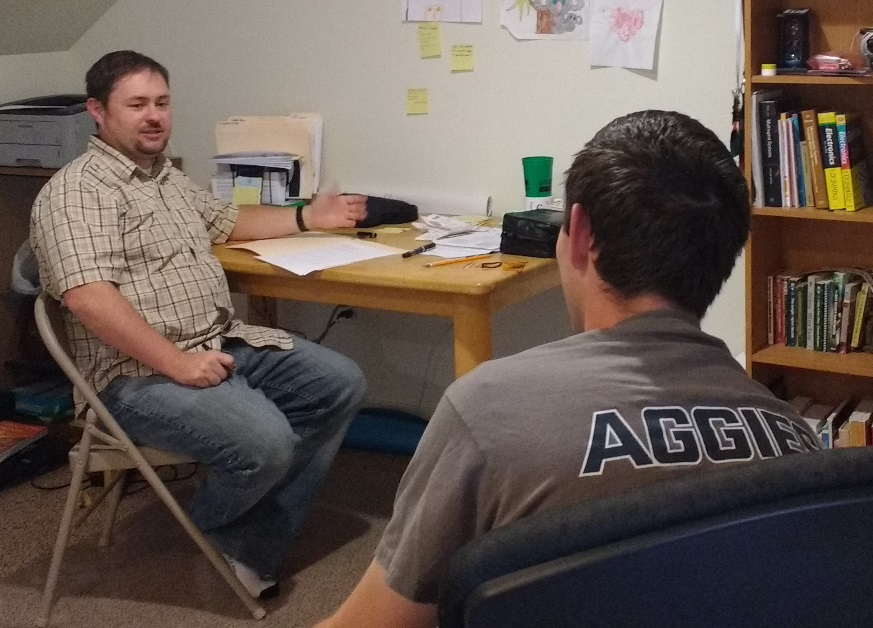
\includegraphics[width=0.9\marginparwidth]{figures/user_study.jpg}
	\caption{A user study was undertaken as semi-structured one-on-one
	  interviews with 12 subjects.}
  \end{minipage}
\end{marginfigure}



Interview questions allowed us to learn about the typical student's study
habits, explore their prior experiences, and discover their disposition towards
to being part of such a group. By first understanding the motivation behind a
student's decision to reach out for help, we would then better be able to
create a useful application that would actually be adopted.

Semi-structured interviews were performed with twelve participants from various
universities.  Each member of the research team conducted one-on-one interviews
which were carried out in-person or electronically.  Interviews lasted between
twenty and thirty minutes following a common interview template. The
interviewer had the discretion to adapt the discussion so as to probe deeper
into any interesting subject that arose.  All but one of the students
interviewed were undergraduate students.  Participants' investment in their
education spanned a wide spectrum.


\begin{figure}
  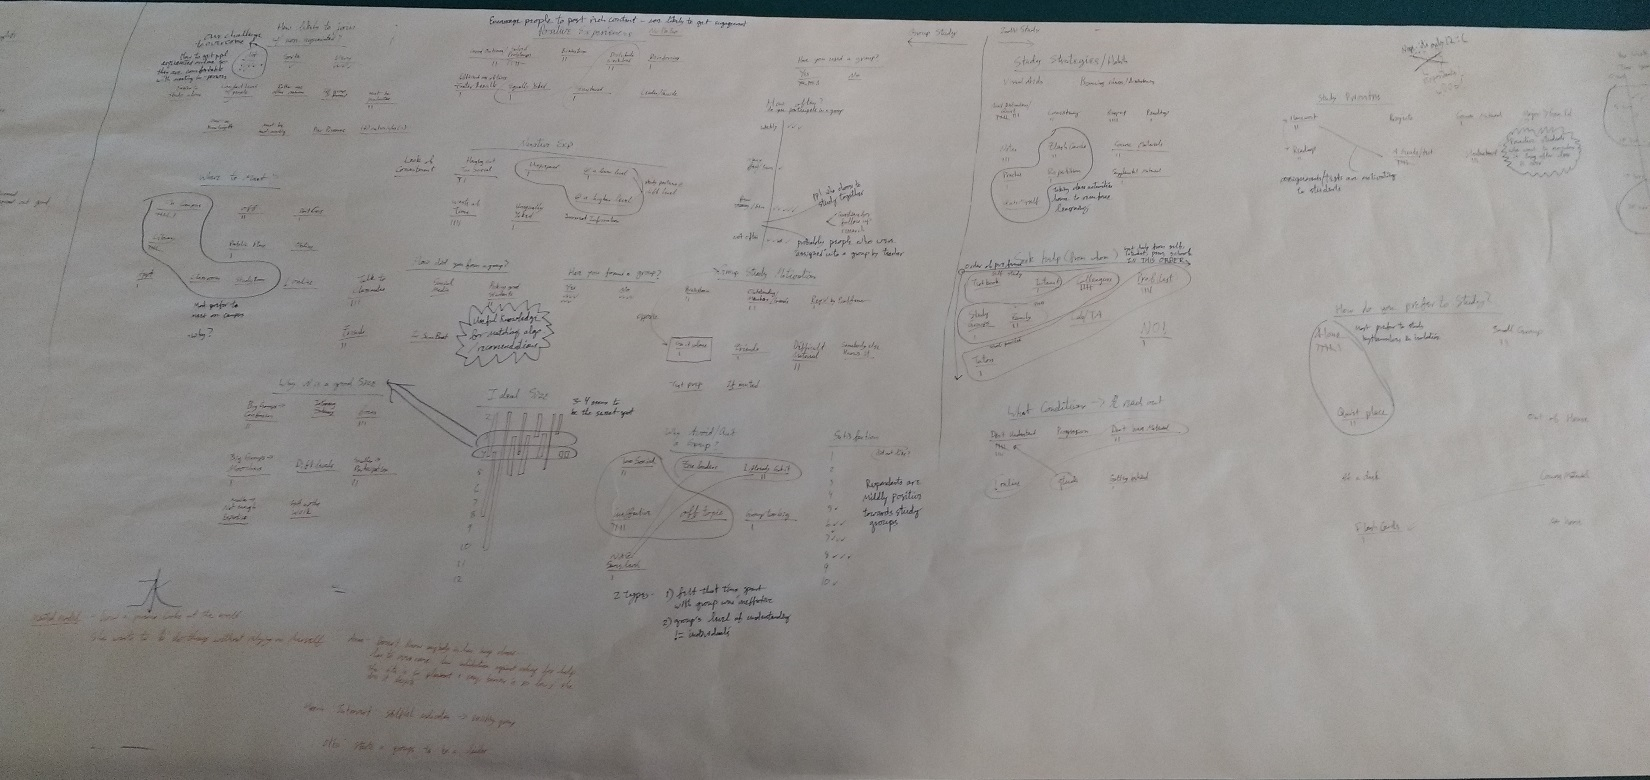
\includegraphics[width=0.9\columnwidth]{figures/affinity_diagram.jpg}
  \caption{Affinity diagram}~\label{fig:sample}
\end{figure}

Interview results were transferred to an affinity diagram to reveal patterns,
commonalities and outliers among the responses.  Respondents were distributed
into two clusters: those who spent little time on study (less than 10 hours per
week) and those making a significant investment (15 to 20 hours per week).
Nearly all subjects studied alone in a quiet location without distractions. A
majority of respondents reported that they will reach out to other people only
after exhausting written resources including textbooks and the Internet; after
those resources failed help might be sought from classmates before the
instructor was queried as a last resort.

The ideal group size was discovered to be three to four individuals.
Participants reported that large groups lacked focus and that it was less
likely for all members to be at the same level of understanding. Respondents
expressed a strong preference to meet on campus. All participants had
previously been assigned to a study groups by an instructor, which experience
was remembered unpleasantly.

Nevertheless, respondents general attitude toward group study was mildly positive with the
caveat that the group must consist of acquaintances and convene in a familiar
environment.  Consequently, our team shifted its focus toward overcoming ingrained biases and
facilitating successful study experiences in comfortable social situations
through a simple and inviting tool.  


\section{Personas and Scenarios}

\subsection{User Personas}

\begin{marginfigure}[-14pc]
  \begin{minipage}{\marginparwidth}
    \centering
  
\includegraphics[width=0.9\marginparwidth]{figures/anna.png}
    \caption{Persona \#1: Outgoing freshman Anna Redder}
  \end{minipage}
\end{marginfigure}

\begin{marginfigure}[0pc]
  \begin{minipage}{\marginparwidth}
    \centering
  
\includegraphics[width=0.7\marginparwidth]{figures/marvin.png}
    \caption{Persona \#2: Introverted non-traditional student Marvin Nivram }
  \end{minipage}
\end{marginfigure}

\begin{marginfigure}[0pc]
  \begin{minipage}{\marginparwidth}
    \centering
  
\includegraphics[width=0.9\marginparwidth]{figures/otto.png}
    \caption{Persona \#3: Aspiring professor Otto von Nov}
  \end{minipage}
\end{marginfigure}




To aid our development of Study Social, personas were derived from our user
research findings to represent an inclusive range of typical students.

\textit{Anna Reeder} is a student who is just embarking on her university education at a
school far from home. She is still in the exploration phase of education as she
learns which areas of study appeal to her.  She has something to prove, which
drives her to take the daring step to attend an out-of-state school to find
what else the world has for her.

\textit{Marvin Nivram} is near the end of his undergraduate studies. Thus he
focuses his schedule on the remaining major courses necessary to complete his
degree. Meanwhile, he is striving to balance his responsibilities as a student
and a husband while living in his parents' basement. Marvin worries that his
introverted nature and uneasiness in social situations will negatively impact
him when it comes time to obtain a ``real'' job upon graduation.

\textit{Otto Von Nov} is a graduate student from Germany who is motivated to
participate in study groups to further his immersion into a new culture.  He
willingly seeks opportunities to improve his mastery of the English language
and to develop the skills that will help him to be successful as a professor.

These personas enabled us to empathize with and consider the full demographic
spectrum of our investigation participants, their varied personalities and
living situations.

\subsection{Scenarios}

Having in mind typical Study Social users, scenarios were devised to give
insight into the conditions which would encourage a user use the application
and how it might aid them.

Two scenarios addressed the reasons cited by participants for \textit{not}
participating in study groups. One scenario sees students placed by their
instructor into an arbitrary group. Not having control over the formation of
the group is demotivating, but use of the application by participants is found
to reduce social anxiety, improve intra-group communication and contribute to
positive group dynamics.

A related scenario exhibits students who recognize the benefits of study groups
despite being uncomfortable with the level of social engagement they entail.
Use of the app helps them to be able to develop important social and job skills
with the intent to improve their marketability to future employers.

The final situation suggested by our user research subjects was that of not
being able to understand or solve material on their own. This nearly universal
experience was cited by many participants as being a strong motivation to
expand their efforts beyond their immediate circle of acquaintances.  Another
scenario described students who wished to form a group but lacked the tools
necessary to do so. 

Taken together, these three scenarios adequately cover the data collected by
our research efforts on overcoming the negative stigma and experiences that are
associated with group studying.



\section{Prototypes}

\subsection{Paper Prototype}

Our design process began by sketching several concepts out on paper. We refined
these sketches through a number of iterations, all the while keeping in balance
competing design considerations.

Working on paper allowed us to quickly explore several diverse structures and
layouts until we found one which we felt would be simple and intuitive. At this
stage we focused on design principles such as ease of exploration and simplicity.
Knowing the time pressures which students face, we aimed to craft an experience
that wold be fun, inviting and, above all, efficient. We reasoned that a
demanding interface would be a turn off to the busy students we are trying to
reach.

\begin{marginfigure}[-24pc]
  \begin{minipage}{\marginparwidth}
    \centering
	  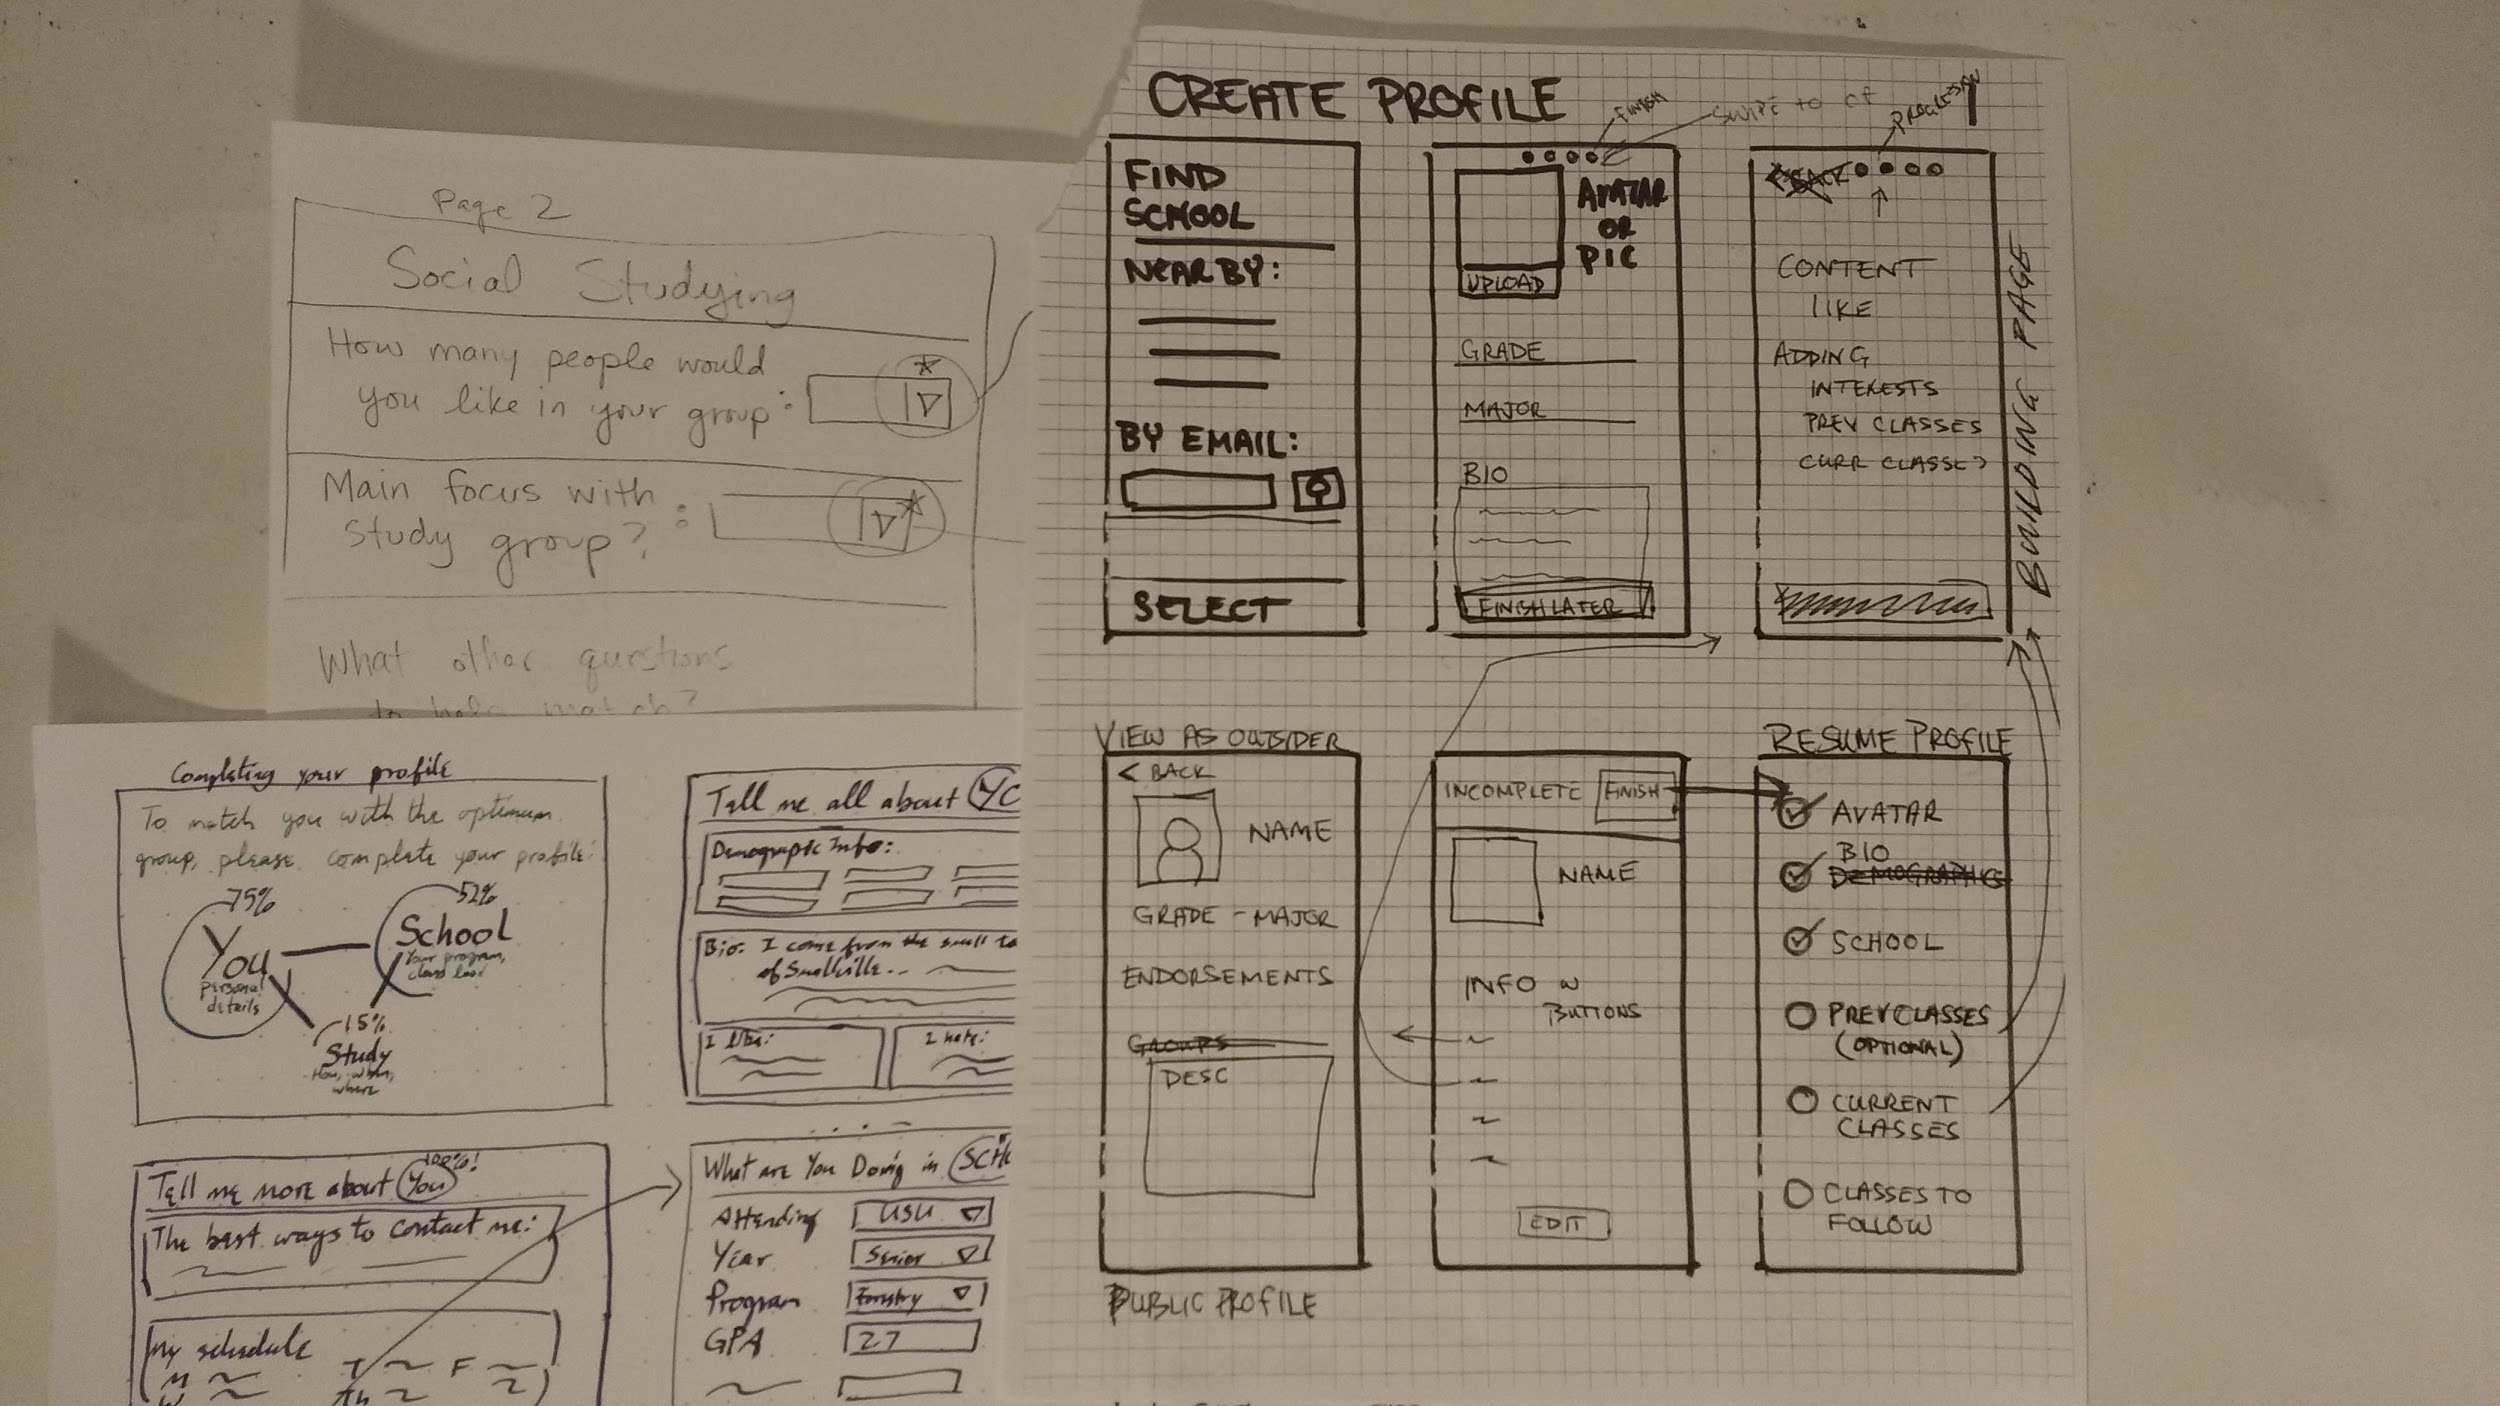
\includegraphics[width=0.7\marginparwidth]{figures/paper_prototype.jpg}
    \caption{Early concept sketches}
  \end{minipage}
\end{marginfigure}



\subsection{Digital Prototype}

\begin{marginfigure}[-7pc]
	\begin{minipage}{\marginparwidth}
		\centering
		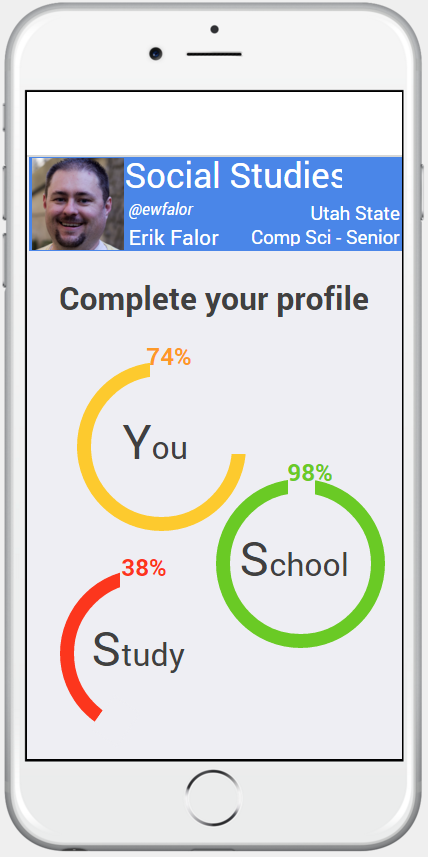
\includegraphics[width=0.9\columnwidth]{figures/prototype1.png}
		\caption{Profile landing page of the initial prototype}~\label{fig:prototype}
	\end{minipage}
\end{marginfigure}


After settling on a concept we created a digital prototype using the JustInMind Prototyping
tool~\cite{justinmind}. This software program enabled our team to create a hi-fidelity interactive
prototype with the ease of making a drawing. The JustInMind Prototyping tool supplies built-in
templates for designing both desktop and mobile applications. Realizing that digital content is
mostly consumed on mobile devices, we focused our efforts on creating a mobile prototype. With this
tool we were quickly able to produce a working prototype which brought to life our paper drawings.


\subsection{Cognitive Walk-through}

Members of our team guided four participants through a cognitive walk-through
evaluation. Participants were asked to complete a few simple, pre-defined tasks
using the digital prototype from a web browser. Having an interactive
web-based prototype made administering the cognitive walk-through simple owing
to the fact that our test subjects were already comfortable with the concept of
a webpage and could begin tackling their assigned tasks with minimal prompting.

The cognitive walk-through revealed weaknesses in our design which we had
theretofore been blind to. One such revelation was that our navigation scheme
was insufficient and inconsistent, leaving users lost and confused.  This
design deficit followed from our understanding of how a paper prototype ought
to be designed. Looking back, it is clear that we had come to envision the
application as a sequence of hyperlinked pages, one screen in size instead of
imagining it as a unified, continuous flow.  Navigation was unnecessarily
difficult because it wasn't always clear on which screen a piece of desired
information was located, nor was it obvious how to reach a desired destination
from the user's current screen.

Another issue reported by a majority of participants was inadequate feedback.
An oft-cited complaint was that after painstakingly entering data into the
mobile application via an on-screen keyboard, there was no "save" button
provided. Navigating back to the previous screen did not reassure the user that
their data was saved. Nor was there any indication of an autosave feature.
Because of this users sought in vain for the missing button and were reluctant
to leave the page containing the text-entry forms.



\subsection{Heuristic evaluation}

Following the cognitive walk-through our team performed a heuristic evaluation on the most important
functions of the application. Of the ten design heuristics under consideration, two repeatedly came
up as problematic to our prototype. These were ``User control and freedom'' and ``consistency and
standards''. The aforementioned navigation confusion along with the lack of a save button were the
biggest drivers of the former heuristic. The latter was exemplified by our inconsistent use of
navigation hints and a complicated search interface.



\section{Usability Testing}

The result of the foregoing evaluation activities was a bottom-up redesign of
our application prototype which was prepared for a usability testing activity.
This usability testing of the application was performed with the assistance of
five volunteers, drawn from the pool of participants of our prior research
activities. As with the cognitive walk-through, the usability testing activity
was performed using the JustInMind Prototyping tool~\cite{justinmind}.  These
users were able to judge the difference between the initial and improved
prototype, and all agreed that the new prototype addressed their concerns.

Users were asked to perform a series of tasks including creating and populating
a personal profile, finding an existing study group and creating a new study
group. Participants vocalized their thoughts and frustrations to give us
insight into a user's experience.


\marginpar{
	\vspace{-180pt}
	\fbox {
		\begin{minipage}{0.925\marginparwidth}
			\textbf{Usability Testing Tasks}
			\begin{itemize}
				\item	Create account
				\item	Edit Profile
				\item	Make Profile Private
				\item	Find and Join Group
				\item	Create new group
			\end{itemize}
		\end{minipage}
	}
}

\begin{marginfigure}[23pt]
  \begin{minipage}{\marginparwidth}
    \centering
	  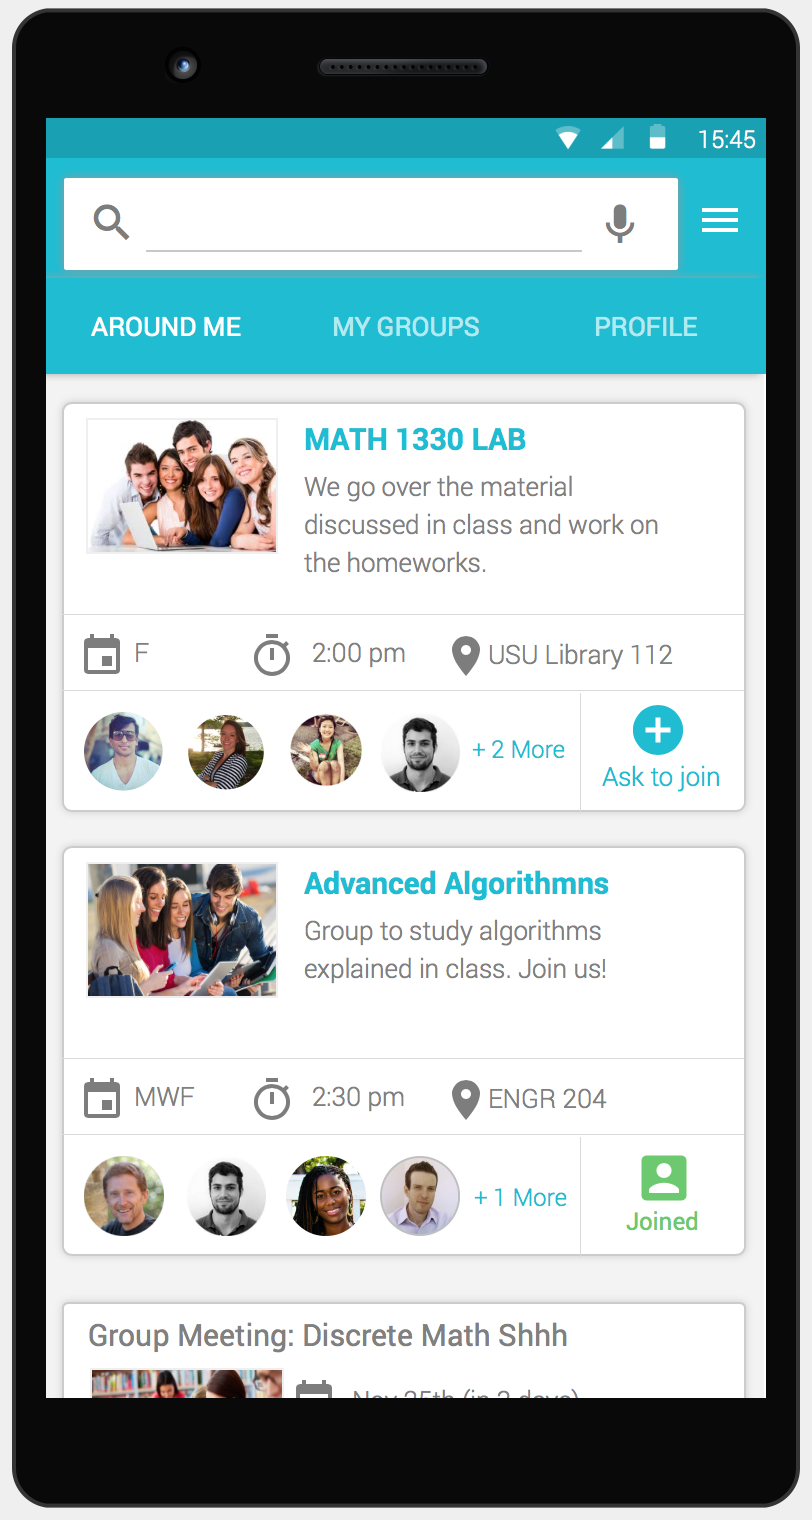
\includegraphics[width=0.7\marginparwidth]{figures/beta_prototype.png}
    \caption{Final prototype}
  \end{minipage}
\end{marginfigure}





\section{Conclusion}

Understanding what prevents students from enjoying effective group study
sessions helped our team create the Study Social application. Our initial group
of interviewees who expressed negative feelings towards group study later
remarked that they would definitely use the product our final prototype
represented.  Evolving our idea from a simple tutor-student matching
application to a complete group collaboration study application with chat and
file uploads was a iterative process led by research.  Study Social is
positioned to fill a niche in the market between a social forming application
and a collaboration tool.  Students can overcome the initial barriers of
forming functioning study groups and improve confidence, understanding,
accuracy, and overcome frustration by working together on difficult material.        


\section{Acknowledgements}

We are grateful to all of the participants who
volunteered through interviews, cognitive walk-throughs, usability tests and in
other activities. Their input was invaluable and really helped this project
take shape.  We owe a debt of gratitude to our helpful and enthusiastic mentor
and advisor, Dr. Amanda Hughes. We could never have created such a successful
prototype without her brilliant insight and helpful advice.  Some of the
references cited in this paper are included for illustrative purposes only.



\balance{}

% \bibliographystyle{ACM-Reference-Format-Journals}
\bibliographystyle{SIGCHI-Reference-Format}
% \bibliographystyle{acm}
\bibliography{Team-FTW-Report}

\end{document}

%%% Local Variables:
%%% mode: latex
%%% TeX-master: t
%%% End:
